\section{Theorie}
\label{sec:Theorie}
In dem Versuch sollen das Emissionsspektrum einer Cu-Röntgenröhre und verschiedene Absorptionsspektren aufgenommen und analysiert werden.
\\
Um Röntgenstrahlung zu erzeugen werden in einer evakuierten Röhre aus einer Glühkathode Elektronen emittiert und auf eine Anode hin beschleunigt. 
Die Röntgenstrahlung entsteht wenn die Elektronen auf die Anode treffen. Dabei besteht die entstandene Röntgenstrahlung aus dem kontinuierlichen
 Bremsspektrum, so wie aus der charakteristischen Röntgenstrahlung des Anodenmaterials. 
 Bei der Abbremsung eines Elektrons im Coulombfeld des Atomkerns wird ein Photon emittiert, dessen Energie dem Energieverlust des abgebremsten Elektrons entspricht.
 Da das Elektron sowohl eine Teilenergie als auch seine Gesamtenergie abgeben kann, handelt es sich beim Bremsspektrum um ein kontinuierliches Spektrum (Abbildung \ref{fig:Brems}).
 \begin{figure}
    \centering
    \caption{Typisches Bremssprektrum \cite{}}
    \label{fig:Brems}
    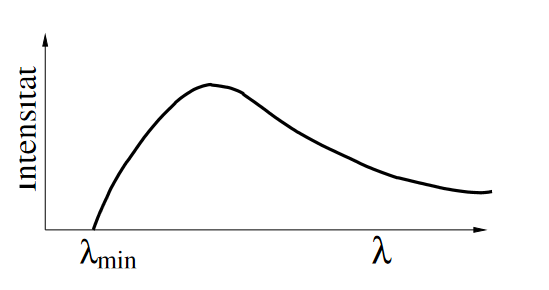
\includegraphics[width = 0.6 \textwidth]{pics/Bremsspe.png}
\end{figure}
 Die minimale Wellenlänge 
 \begin{equation}
     \lambda_\text{min}=\frac{h c}{e_0 U}
     \label{eqn:lammin}
 \end{equation}
 wird bei der vollständigen Abbremsung des Elektrons erreicht.
 Dabei beschreibt $h$ das Plancksche Wirkungsquant, $c$ die Lichtgeschwindigkeit und $e_0 U$ die gesamte kinetische Energie des Elektrons.
 Die charakteristische Röntgenstrahlung wird durch das Anodenmaterial bestimmt. Diese entsteht bei der Ionisierung des Atoms, wodurch ein Elektron aus einer äußeren Schale in die innere Schale zurückfällt.
 Dabei wird ein Röntgenquant mit der Energie der Energiedifferenz $h \nu = E_\text{m}-E_\text{m}$ der beiden Energieniveaus emittiert. Es entstehen scharfe Linien die mit $K_\alpha, K_\beta, L_\alpha, ...$ 
 bezwichnet werden. Dabei sind die Buchstaben K, L, M, ... die Schalen des Atoms, auf der die Übergänge enden. Der griechische Buchstabe gibt an aus welcher Schale das Elektron stammt welches die Innere Schale auffüllt.
 Bei einem Mehrelektronenatom wird die Kernladung durch die Hüllenelektronen und die Wechselwirkung der Elektronen abgeschirmt. Durch die Verringerung der Coulomb Anziehung auf das äußere Elektron, ergibt sich 
 \begin{equation}
     E_\text{n}=-R_{\inf} z_\text{eff}^2 \frac{1}{n^2}
     \label{eqn:Bindungse}
 \end{equation}
 für die Bindungsenergie $E_\text{n}$ eines Elektrons auf der n-ten Schale. Hierbei ist $R_{\inf}=\SI{13.6}{\electronvolt}$ und $z_\text{eff}=z - \sigma$ die effektive Kernladung mit $\sigma$ als Abschirmkonstante.
 Die Abschirmkonstante unterscheidet sich für jedes Elektron und ist  empirisch bestimmbar. Die Elektronen besitzen neben der Hauptquantenzahl noch weitere Quantenzahlen resultierend aus dem Elektronenspin und dem Bahndrehimpuls, so dass eine Feinstruktur ersichtlich wird.
 Die Energien dieser Feinstruktur können mithilfe der Sommerfeldschen Feinstrukturformel 
 \begin{equation}
     E_\text{n,j}=-R_{\inf} \left(z_\text{eff}^2 \frac{1}{n^2} + \alpha^2 z_\text{eff}^4 \frac{1}{n^3} \left(\frac{1}{j+\frac{1}{2}} - \frac{3}{4n}\right) \right)
     \label{eqn:sommerfeld}
 \end{equation}
ermittelt werden. Wobei $\alpha$ die Sommerfeldsche Feinstrukturkonstante, n die Hauptquantenzahl und j der Gesamtdrehimpuls des betrachteten Elektrons ist.
\\
Charakteristische Röntgenstrahlung tritt auch bei Absorption von Röntgenstrahlung durch einen Absorber auf. Bei Energien unter $\SI{1}{\mega \electronvolt}$
treten der Comptoneffekt so wie der Photoeffekt dominant auf. Wie in Abbildung \ref{fig:abso} zu sehen, nimmt der Absorptionskoeffizient mit zunehmender Energie ab und wenn die Photonenenergie gerade größer ist als die Bindungsenergie eines Elektrons aus der nächsten Schale steigt er Sprunghaft an.
\begin{figure}
    \centering
    \caption{Absorptionsspektrum von Röntgenstrahlung \cite{}}
    \label{fig:abso}
    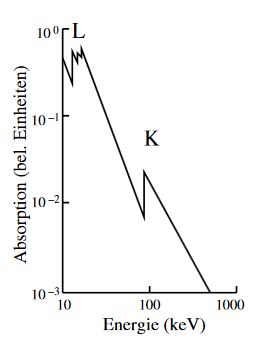
\includegraphics[width = 0.6 \textwidth]{pics/abso.png}
\end{figure}
Die Absorptionskanten haben nahezu die selben Energien wie die Bindungsenergie des Elektrons $h \nu_\text{abs}= E_\text{n} - E_{\inf}$. Die zugehörige Energie wird nach der zugehörigen Schale aus denen das Elektron stammt als K-, L-, M-, ... Absorptionskante bezeichnet. 
Mit hilfe der Sommerfeldschen Feinstrukturformel kann die Abschirmkonstante mit
\begin{equation}
    \sigma_\text{K}=Z-\sqrt{\frac{E_\text{K}}{R_{\inf}}-\frac{\alpha^2 Z^4}{4}}
    \label{eqn:abschirmkonstante}
\end{equation}
bestimmt werden. Der zweite Term unter der Wurzel berücksichtigt dabei die Feinstrukturaufspaltung der K-Schale.\\
Durch Benutzen der Bragg'schen Reflexion kann die Energie bzw. die Wellenlänge $\lambda$ der Röntgenstrahlung experimentell analysiert werden.
Hierbei fällt Röntgenlicht auf ein dreidimensionales Gitter, wobei die Photonen an jedem Atom des Gitters gebeugt werden. Die Strahlen interferieren und unter dem Glanzwinkel $\theta$ 
kommt es zu konstruktiver Interferenz. So kann mit hilfe der Bragg'schen Bedingung
\begin{equation}
    2 d \sin \theta = n \lambda
    \label{eqn:bragg}
\end{equation}
und einer bekannten Gitterkonstante d ($d_\text{Lif}=\SI{201.4}{\pico \metre}$) die Wellenlänge bestimmt werden. Dabei ist n die Beugungsordnung des Maxima.
